%%%%%%%%%%%%%%%%%%%%%%%%%%%%%%%%%%%%%%%%%%%
%
% From a template maintained at https://github.com/jamesrobertlloyd/cbl-tikz-poster
%
% Code near the top should be fairly standard and not need to be changed
%  - except for the document class
% Code lower down is more likely to be customised
%
%%%%%%%%%%%%%%%%%%%%%%%%%%%%%%%%%%%%%%%%%%%

%%%%%%%%%%%%%%%%%%%%%%%%%%%%%%%%%%%%%%%%%%%
%
% Document class
%
% Change this if you want a different size / orientation poster etc
%
%%%%%%%%%%%%%%%%%%%%%%%%%%%%%%%%%%%%%%%%%%%

\documentclass[landscape,a0b,final,a4resizeable]{a0poster}
%\documentclass[portrait,a0b,final,a4resizeable]{a0poster}

%%%%%%%%%%%%%%%%%%%%%%%%%%%%%%%%%%%%%%%%%%%
%
% 'Basic' packages
%
% TODO - Almost certainly some are unnecessary - feel free to remove nonstandard
% packages if you think it is a good idea not to always have them
%
%%%%%%%%%%%%%%%%%%%%%%%%%%%%%%%%%%%%%%%%%%%
\usepackage{graphicx}
% \usepackage[draft]{graphicx}
\graphicspath{ {fig/} }
 \usepackage[export]{adjustbox}
 
\usepackage{todonotes}
\usepackage[inline]{enumitem}
\usepackage{bm}

\usepackage{sty/msoelch/mlmacros}
\usepackage{amsmath}
\usepackage{mathtools}
\usepackage{calc}
\usepackage{fontawesome}
\usepackage{hyperref}

%\usepackage[osf,sc]{mathpazo} % Palatino as the main font
%\linespread{1.05}\selectfont % Palatino needs some extra spacing, here 5% extra
% \usepackage[euler-digits]{eulervm} % nicer math font

% \usepackage{floatrow}
\usepackage[skip=5pt]{caption}
\usepackage{subcaption}

\usepackage[noabbrev]{cleveref}

% section spacing
\usepackage{titlesec}

\titlespacing*{\section}
{0pt}{.1\baselineskip}{.1\baselineskip}
  
% Decrease spacing between bib entries
%\setlength{\bibsep}{0pt plus 0.3ex}

\newcommand*{\B}[1]{\ifmmode\bm{#1}\else\textbf{#1}\fi}

\variables{a,b,c,g,t,o,s,v,x,z}
\variables{A,I}

\variables[app]{\alpha}
\variables[mean]{\mu}
\variables[std]{\sigma}
\variables[map]{\nu}
\variables[dparam]{\psi}

% Neil's comment function
\newcommand{\nd}[1]{\textcolor{red}{[ND: #1]}}
\newcommand{\ab}[1]{\textcolor{green}{[AB: #1]}}
\newcommand{\ak}[1]{\textcolor{blue}{[AK: #1]}}

\probdists{p,q}

\DeclarePairedDelimiter{\fences}{(}{)}
\DeclarePairedDelimiter{\norm}{\lVert}{\rVert}

%\DeclareMathOperator{\MLP}{ \mathrm{MLP} \Fences }
\newcommand{\MLP}[1]{ \mathrm{MLP} \fences{#1} }
\newcommand{\LSTM}[1]{ \mathrm{LSTM} \fences{#1} }
\newcommand{\flatten}[1]{ \mathrm{vec} \fences{#1} }

\newcommand{\reg}[1]{ \ensuremath{R} \fences{#1} }

\definecolor{darkgreen}{rgb}{0,.502,0}

\newcommand{\sidecaption}[1]% #1 = label name
{\raisebox{\abovecaptionskip}{\begin{subfigure}[t]{1.6em}
  \caption[singlelinecheck=off]{}% do not center
  \label{#1}
\end{subfigure}}\ignorespaces}

\usepackage{multicol}
\usepackage{color}
\usepackage{shadow}
\usepackage{morefloats}
\usepackage{cite}
%\usepackage[pdftex]{graphicx}
\usepackage{rotating}
\usepackage{amsmath, amsthm, amssymb, bm}
\usepackage{array}
\usepackage{nth}
\usepackage[square,numbers]{natbib}
\usepackage{booktabs}


%%%%%%%%%%%%%%%%%%%%%%%%%%%%%%%%%%%%%%%%%%%
%
% TIKZ packages and common definitions
%
% Add extra things as per your tikz needs
%
%%%%%%%%%%%%%%%%%%%%%%%%%%%%%%%%%%%%%%%%%%%

\usepackage{../common/picins}
\usepackage{tikz}
\usetikzlibrary{shapes.geometric,arrows,chains,arrows.meta,matrix,positioning,scopes,calc}
\tikzstyle{mybox} = [draw=none, rectangle]

%%%%%%%%%%%%%%%%%%%%%%%%%%%%%%%%%%%%%%%%%%%
%
% myfig
%
% \myfig - replacement for \figure
% necessary, since in multicol-environment 
% \figure won't work        
%                 
%%%%%%%%%%%%%%%%%%%%%%%%%%%%%%%%%%%%%%%%%%%

\newcommand{\myfig}[3][0]{
\begin{center}
  \vspace{1.5cm}
  \includegraphics[width=#3\hsize,angle=#1]{#2}
  \nobreak\medskip
\end{center}}

%%%%%%%%%%%%%%%%%%%%%%%%%%%%%%%%%%%%%%%%%%%
%
% mycaption                
%
% \mycaption - replacement for \caption
% necessary, since in multicol-environment \figure and
% therefore \caption won't work
%
%%%%%%%%%%%%%%%%%%%%%%%%%%%%%%%%%%%%%%%%%%%

%\newcounter{figure}
\setcounter{figure}{1}
\newcommand{\mycaption}[1]{
  \vspace{0.5cm}
  \begin{quote}
    {{\sc Figure} \arabic{figure}: #1}
  \end{quote}
  \vspace{1cm}
  \stepcounter{figure}
}

%%%%%%%%%%%%%%%%%%%%%%%%%%%%%%%%%%%%%%%%%%%
%
% Some standard colours
%
%%%%%%%%%%%%%%%%%%%%%%%%%%%%%%%%%%%%%%%%%%%

\definecolor{oriblue}{cmyk}{1., .8, 0., .6}
\definecolor{camlightblue}{rgb}{0.601 , 0.8, 1}
\definecolor{camdarkblue}{rgb}{0, 0.203, 0.402}
\definecolor{camred}{rgb}{1, 0.203, 0}
\definecolor{camyellow}{rgb}{1, 0.8, 0}
\definecolor{lightblue}{rgb}{0, 0, 0.80}
\definecolor{white}{rgb}{1, 1, 1}
\definecolor{whiteblue}{rgb}{0.80, 0.80, 1}

%%%%%%%%%%%%%%%%%%%%%%%%%%%%%%%%%%%%%%%%%%%
%
% Some look and feel definitions
%
%%%%%%%%%%%%%%%%%%%%%%%%%%%%%%%%%%%%%%%%%%%

\setlength{\columnsep}{0.03\textwidth}
\setlength{\columnseprule}{0.0018\textwidth}
\setlength{\parindent}{0.0cm}

%%%%%%%%%%%%%%%%%%%%%%%%%%%%%%%%%%%%%%%%%%%
%
% \ - replacement for \section*
% 
% Puts a pretty box around some text
% TODO - any other thoughts for what this box should look like
%
%%%%%%%%%%%%%%%%%%%%%%%%%%%%%%%%%%%%%%%%%%%

\tikzstyle{mysection} = [rectangle, 
									draw=none, 
									shade, 
									outer color=oriblue,
									inner color=oriblue,
									text width=0.965\columnwidth,
									text centered,
									rounded corners=20pt,
									minimum height=0.11\columnwidth]

\newcommand{\mysection}[1]
{
\begin{center}
  \begin{tikzpicture}
    \node[mysection] {\textcolor{white}{\sffamily\bfseries\LARGE#1}};
  \end{tikzpicture}
\end{center}
}

%%%%%%%%%%%%%%%%%%%%%%%%%%%%%%%%%%%%%%%%%%%
%
% Set the font
%
% TODO - Not sure what a canonical choice is - feel free to modify
%
%%%%%%%%%%%%%%%%%%%%%%%%%%%%%%%%%%%%%%%%%%%

\renewcommand{\familydefault}{cmss}
\sffamily

%%%%%%%%%%%%%%%%%%%%%%%%%%%%%%%%%%%%%%%%%%%
%
% Poster environment
%
% Centres everything and can be used to define the width of the content
%
%%%%%%%%%%%%%%%%%%%%%%%%%%%%%%%%%%%%%%%%%%%

\newenvironment{poster}{
  \begin{center}
  \begin{minipage}[c]{0.96\textwidth}
}{
  \end{minipage} 
  \end{center}
}

%%%%%%%%%%%%%%%%%%%%%%%%%%%%%%%%%%%%%%%%%%%
%
% This is probably a good place to put content specific packages and definitions
%
%%%%%%%%%%%%%%%%%%%%%%%%%%%%%%%%%%%%%%%%%%%

\newtheorem{thm}{Theorem}%[section]
\newtheorem{lem}[thm]{Lemma}
\newtheorem{prop}[thm]{Proposition}
\newtheorem{cor}[thm]{Corollary}

\newtheorem*{theorem*}{Theorem}

\theoremstyle{definition}
\newtheorem*{definition*}{Definition}
\newtheorem{definition}[thm]{Definition}%[section]
\newtheorem{conj}{Conjecture}[section]
\newtheorem{exmp}{Example}[section]
\newtheorem{rem}[thm]{Remark}

\theoremstyle{remark}
%\newtheorem{rem}{Remark}
\newtheorem{note}{Note}
\newtheorem{case}{Case}

\newcommand{\eqd}{\overset{\,_{\!d}}{=}}
\newcommand{\defn}[1]{\emph{#1}}

\newcommand{\Law}{\mathcal{L}}

\def\given{\,|\,}

\def\SGinf{\mathbb{S}_{\infty}}

\newcommand{\NonNegInts}{\mathbb{Z}_+}
\newcommand{\Nats}{\mathbb{N}}
\newcommand{\Rationals}{\mathbb{Q}}
\newcommand{\Reals}{\mathbb{R}}

\newcommand{\as}{\textrm{a.s.}}

\def\[#1\]{\begin{align}#1\end{align}}
\newcommand{\defas}{:=}

\newcommand{\Normal}{\mathcal{N}}
\newcommand{\dist}{\ \sim\ }

\newcommand{\kernel}{\kappa}
\newcommand{\kernelmatrix}{K}
\newcommand{\scalefactor}{s}
\newcommand{\lengthscale}{\ell}
\newcommand{\targets}{T}
\newcommand{\noise}{\sigma_\targets}
\newcommand{\pseudopoints}{\eta}
\newcommand{\inputpoints}{\xi}
\newcommand{\covhyppar}{\psi}
\newcommand{\logistic}{\phi}

\newcommand{\CompOrder}{\mathcal{O}}
\def\graphspace{\mathbf{G}}
\def\Uniform{\mbox{\rm Uniform}}
\def\Bernoulli{\mbox{\rm Bernoulli}}
\def\ie{i.e.,\ }
\def\eg{e.g.,\ }
\def\iid{i.i.d.\ }
\def\simiid{\sim_{\mbox{\tiny iid}}}
\def\simind{\sim_{\mbox{\tiny ind}}}
\def\eqdist{\stackrel{\mbox{\tiny d}}{=}}
\def\ahfunction{\theta}       
\def\AHfunction{\Theta}           % A-H random function
\def\AHvar{U}                     % A-H uniform variables
\def\AHvaralt{V}                  % A-H uniform variables - for bipartite data
\def\larray{W}                    % latent array sampled with A-H
%\def\latentspace{\mathbf{W}}      % range of entries
\def\latentspace{\mathcal{W}}      % range of entries
\def\darray{X}                    % data array
%\def\dataspace{\mathbf{X}}        % sample space
\def\dataspace{\mathcal{X}}        % sample space
\def\cfspace{\mathbf{C}}          % space of continuous functions
%\def\GP{\mbox{\mathcal{GP}}}
\def\GP{\mathcal{GP}}
\def\likelihood{P}
\def\CovData{C}
\def\CovDataAlt{D}

\def\newarrow{\mbox{\begin{tikzpicture}
             \useasboundingbox{(-3pt,-4.5pt) rectangle (19pt,1pt)};
             \draw[->] (0,-0.07)--(17pt,-0.07);\end{tikzpicture}}}
         
%%%%%%%%%%%%%%%%%%%%%%%%%%%%%%%%%%%%%%%%%%%
%
% The document environment starts here
%
%%%%%%%%%%%%%%%%%%%%%%%%%%%%%%%%%%%%%%%%%%%

\begin{document}

%%%%%%%%%%%%%%%%%%%%%%%%%%%%%%%%%%%%%%%%%%%
%
% Begin the poster environment - centres things and potentially changes the width
%
%%%%%%%%%%%%%%%%%%%%%%%%%%%%%%%%%%%%%%%%%%%

\begin{poster}

%%%%%%%%%%%%%%%%%%%%%%%%%%%%%%%%%%%%%%%%%%%
%
% Potentially add some space at the top of the poster
%
%%%%%%%%%%%%%%%%%%%%%%%%%%%%%%%%%%%%%%%%%%%

\vspace{0\baselineskip}

%%%%%%%%%%%%%%%%%%%%%%%%%%%%%%%%%%%%%%%%%%%
%
% Draw the header as a TIKZ picture
%
% Using TIKZ to allow for easy alignment
%
%%%%%%%%%%%%%%%%%%%%%%%%%%%%%%%%%%%%%%%%%%%

\begin{center}
\begin{tikzpicture}[x=0.5\textwidth]
    % Dummy nodes at edges for spacing
    % TODO - a better way?
    \node at (+1, 0) {};    
    \node at (-1, 0) {};
    % Set the size of the badges
    \def \badgeheight {0.06\textwidth}
    % Title text
    \node[inner sep=0,text width=0.5\textwidth,text centered,font=\Huge]
%    \node[inner sep=0,
%    text width=0.5\textwidth,
%    text centered,
%    font=\Huge,
%    draw=none,
%    shade,
%    outer color=oriblue,
%    inner color=oriblue] 
    (Title) at (0,0) 
    {
      {\sffamily \Huge \textbf{Hierarchical Attentive Recurrent Tracking}}\\
      {\huge\sffamily Adam R. Kosiorek, Alexy Bewley, Ingmar Posner}\\
      \vspace{-0.3\baselineskip}
      {\large\sffamily Applied AI Lab, Department of Engineering Science, University of Oxford, UK}
    };
    % Cambridge badge
    \node [mybox] (Cambridge Badge) at (-.7, 0) {
        
\includegraphics[height=\badgeheight]{../badges/a2i_logo.pdf}
    };
    % Columbia logo
    \node [mybox] (box) at (0.7, 0) {
        
\includegraphics[width=0.2\textwidth]{../badges/oxford.pdf}
    };
\end{tikzpicture}
\end{center}

%%%%%%%%%%%%%%%%%%%%%%%%%%%%%%%%%%%%%%%%%%%
%
% Spacing between title and main body
%
%%%%%%%%%%%%%%%%%%%%%%%%%%%%%%%%%%%%%%%%%%%

\vspace{1\baselineskip}

%%%%%%%%%%%%%%%%%%%%%%%%%%%%%%%%%%%%%%%%%%%
%
% Columns environment
%
%%%%%%%%%%%%%%%%%%%%%%%%%%%%%%%%%%%%%%%%%%%

\begin{multicols}{3}

%%%%%%%%%%%%%%%%%%%%%%%%%%%%%%%%%%%%%%%%%%%
%
% Start of content
%
%%%%%%%%%%%%%%%%%%%%%%%%%%%%%%%%%%%%%%%%%%%

\Large

%\mysection{Motivation}
\vspace{2\baselineskip}
\mysection{Hierarchical Attention}

\vspace{2\baselineskip}


    \begin{minipage}[c]{0.3\textwidth}
        \centering
        \begin{subfigure}[b]{1.\textwidth}
            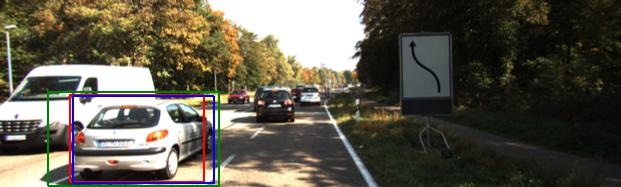
\includegraphics[width=\textwidth]{att_img}
        \end{subfigure}
        
        \hspace{-30pt}
        \begin{minipage}{.85\textwidth}
            \vspace{.5em}
            \begin{subfigure}[b]{.29\textwidth}
                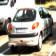
\includegraphics[width=\textwidth, cfbox=darkgreen 4pt 0pt]{att_glimpse}
            \end{subfigure}
            \hfill
            \hspace{8pt}
            \begin{subfigure}[b]{.29\textwidth}
                
\includegraphics[width=\textwidth]{att_mask}
            \end{subfigure}
            \hfill
            \hspace{5pt}
            \begin{subfigure}[b]{.29\textwidth}
                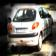
\includegraphics[width=\textwidth]{att_overlay}
            \end{subfigure}
            
        \end{minipage}
    \end{minipage}\hfill
 
    \begin{minipage}[c]{0.3\textwidth}
        \vspace{1em}
            \textcolor{blue}{Ground-truth} and \textcolor{red}{predicted} bounding boxes and an \textcolor{darkgreen}{attention glimpse}. The bottom row shows the three layers of attention: 
            \begin{description}%[labelsep=1em, leftmargin=!,labelwidth=\widthof{\bfseries Interpretable:}]
                \item [$1^{st}$]  layer extracts an attention glimpse (left)
                \item [$2^{nd}$]  layer uses appearance attention to build a location map (middle)
                \item [$3^{rd}$]  layer uses the location map to suppress distractors (right)
            \end{description}
    \end{minipage}
\vspace{1\baselineskip}
\mysection{Loss}
\vspace{.5\baselineskip}
    \centering
    Directly optimise Intersection-over-Union (IoU) and guide attention mechanisms.
%\begin{equation*}
%\loss[\mathrm{HART}]{\cdot} = \lambda_{\mathrm{t}} \loss[\mathrm{t}]{\cdot} + \lambda_{\mathrm{s}} \loss[\mathrm{s}]{\cdot} + \lambda_{\mathrm{a}} \loss[\mathrm{a}]{\cdot}  + \reg{ \B{\lambda} } + \beta \reg{ \cdot }
%\end{equation*}
\begin{equation*}
\loss[\mathrm{HART}]{\cdot} = \lambda_{\mathrm{t}} \loss[\mathrm{t}]{\cdot} + \lambda_{\mathrm{s}} \loss[\mathrm{s}]{\cdot} + \lambda_{\mathrm{a}} \loss[\mathrm{a}]{\cdot} + \beta \reg{ \cdot }
\end{equation*}

\begin{description}[leftmargin=\parindent,labelsep=1em]

\item[Tracking:] Negative log of Intersection-over-Union.
\begin{equation*}
    \loss[\mathrm{t}]{\data, \theta} = \expc[\p{\widehat{\bb}_{1:T}}{\bxTs, \bb_1}]{ -\log \mathrm{IoU} \fences{\widehat{\bb}_t, \bbt}}
\end{equation*}

\item[Spatial Attention:] It follows the object, but shouldn't be too big.
\begin{equation*}
    \loss[\mathrm{s}]{\data, \theta} = \expc[\p{\baTs}{\bxTs, \bb_1}]{ -\log \fences*{\frac{ \bat \cap \bbt }{\mathrm{area}\fences{\bbt}} } -\log \fences { 1 - \mathrm{IoU} \fences{\bat, \bxt} } }
\end{equation*}

\item[Appearance Attention:] Cross-entropy with dynamically created target mask $\tau \fences { \bat, \bbt }$:
$\loss[\mathrm{a}]{\data, \theta} =   \expc[\p{\baTs, \bsTs}{\bxTs, \bb_1}]{ H \fences{ \tau \fences { \bat, \bbt }, \bst  } }$.



\begin{minipage}[c]{.3\textwidth}
    \centering
    \vspace{0.75em}
    \caption*{\large With Appearance Attention Loss: Successful Tracking}
    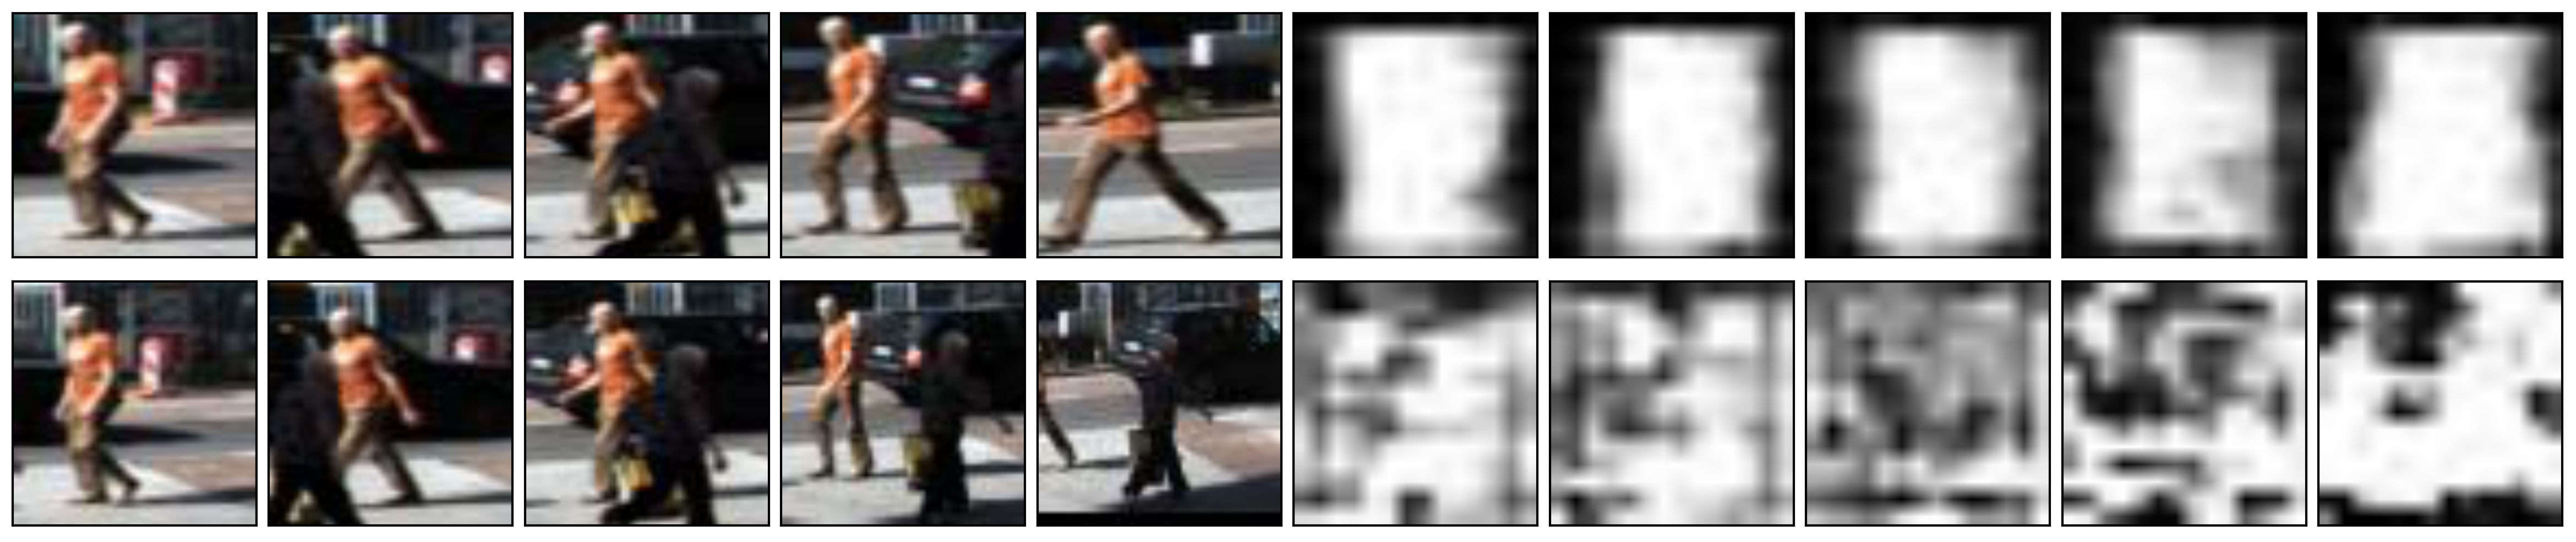
\includegraphics[width=\textwidth]{soft_id_swap}
    \caption*{\large Without Appearance Attention Loss: ID Swap}
\end{minipage}
\end{description}



\newpage

\mysection{Two-stream Attentive Model}

\vspace{.5\baselineskip}

\begin{minipage}[c]{0.3\textwidth}
    \centering
    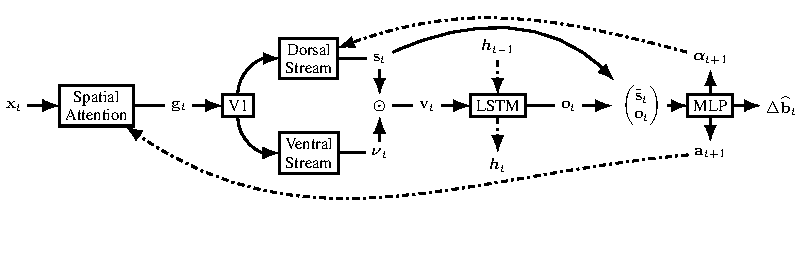
\includegraphics[width=\textwidth]{arch.pdf}
    
    \begin{minipage}[c]{0.5\textwidth}
        \begin{description}
            \item[$\bxt$] input image
            \item[$\bgt$] attention glimpse
            \item[$\bmapt$] appearance-based features
            \item[$\bst$] object segmentation
            \item[$\bvt$] masked features
        \end{description}
    \end{minipage}\hfill
    \begin{minipage}[c]{0.5\textwidth}
                \begin{description}
            \item[$\B{h}_t$] hidden state
            \item[$\bot$] LSTM output
            \item[$\bapp_{t+1}$] appearance
            \item[$\Delta \widehat{\bb}_t$] bounding-box update
            \item[$\ba_{t+1}$] spatial attention
        \end{description}
    \end{minipage}
    
\end{minipage}\hfill

\begin{minipage}{0.3\textwidth}
   \vspace{2em}
   \begin{minipage}[c]{0.5\textwidth}
       \centering
       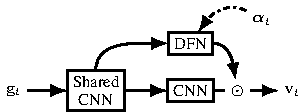
\includegraphics[width=\textwidth]{impl.pdf}
   \end{minipage}\hfill
    \begin{minipage}{0.6\textwidth}
    Appearance attention architecture:
    \vspace{1em}
    \begin{description}[leftmargin=\parindent]
        \item[V1] shared CNN
        \item[Dorsal Stream] Dynamic\\ Filter Network (DFN)
        \item[Ventral Stream] CNN
    \end{description}
    \end{minipage}
\end{minipage}

\vspace{\baselineskip}
%\mysection{Method}

\vspace{0\baselineskip}



\vspace{0\baselineskip}

\mysection{Is Attention Loss Important?}

\vspace{.5\baselineskip}

\centering
\begin{minipage}[c]{.3\textwidth}
    \centering
    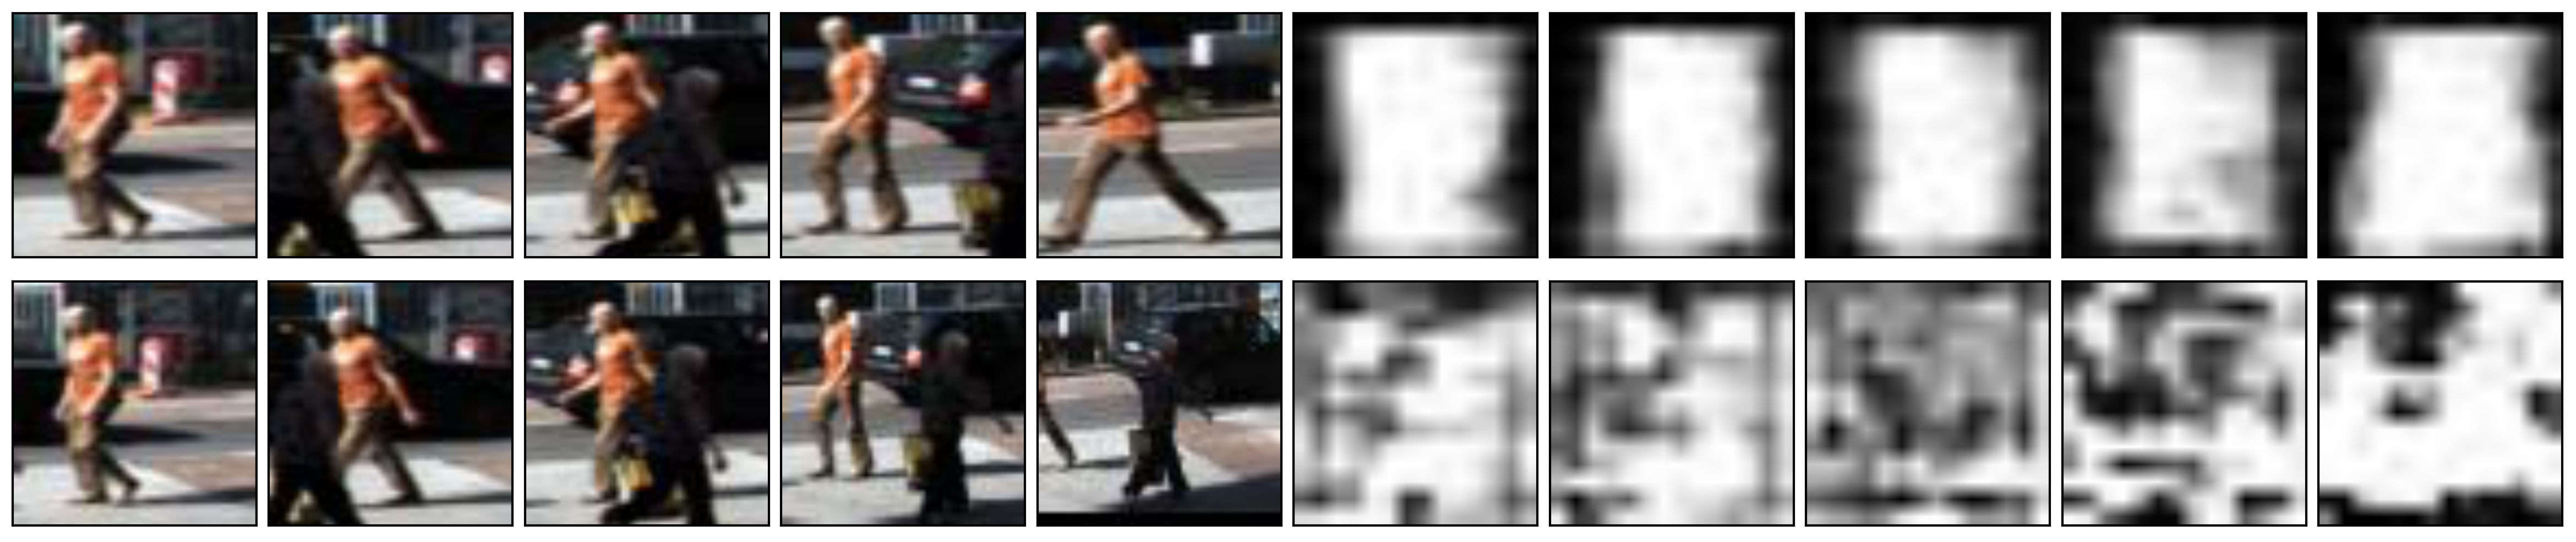
\includegraphics[width=\textwidth]{soft_id_swap}
    \vspace{.5\baselineskip}
    Appearance attention loss (top) prevents an ID swap when a pedestrian is occluded by another one (bottom).
\end{minipage}
\begin{minipage}[c]{.3\textwidth}
    \centering
    \vspace{.5\baselineskip}
    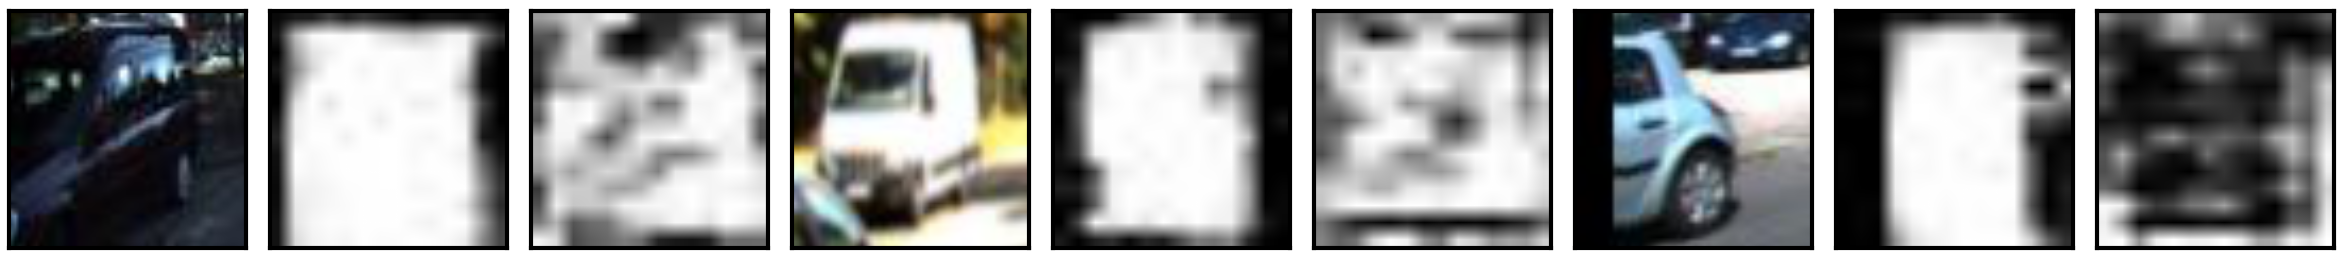
\includegraphics[width=\textwidth]{soft_att}
    \vspace{.5\baselineskip}
   Left to right: glimpses and segmentations learned with and without appearance loss.
   Attention loss leads to distractor suppression. 
\end{minipage}

\vspace{0\baselineskip}


\vspace{.5\baselineskip}

{\large References:}
{\small
\begin{description}
    \item[[1]] Samira Ebrahimi Kahoú, Vincent Michalski, and Roland Memisevic. RATM: Recurrent Attentive Tracking Model. CVPR Work., 2017.
    \item[[2]] Christian Schuldt, Ivan Laptev, and Barbara Caputo. Recognizing human actions: A local SVM approach. In ICPR. IEEE, 2004.
    \item[[3]] A. Geiger, P. Lenz, C. Stiller, and R. Urtasun. Vision meets robotics: The KITTI dataset. Int. J. Rob. Res.,
    32(11):1231–1237, sep 2013.
\end{description}
}

\newpage

\mysection{Pedestrian Tracking: KTH Dataset [2]}

\vspace{1\baselineskip}

\begin{minipage}[c]{0.3\textwidth}
    \centering
    \vspace{-1.5em}
    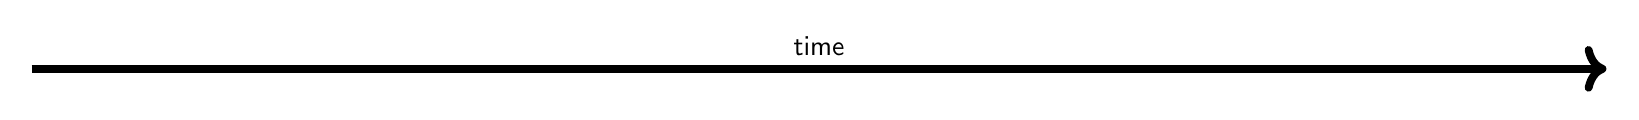
\begin{tikzpicture}
    \draw[line width=1mm, ->] (-10, 0) -- node[above] {time} (10, 0);
    \end{tikzpicture}
    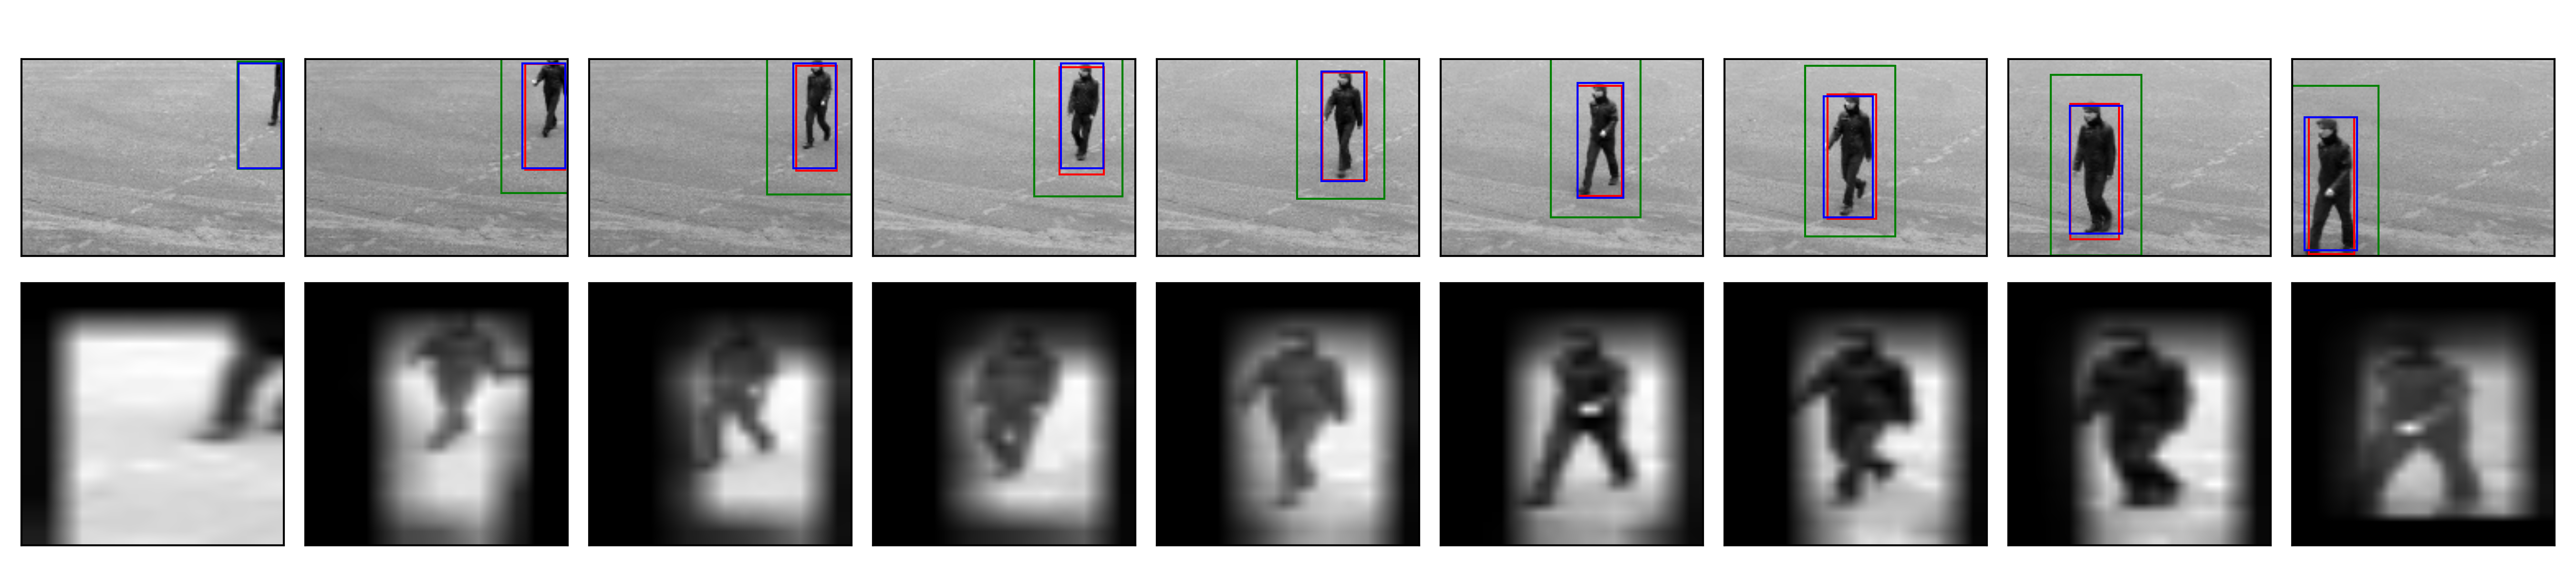
\includegraphics[width=\textwidth]{kth_overlay_16}
    
    \begin{minipage}[c]{0.55\textwidth}
        \begin{itemize}
            \item Attention, prediction and ground-truth overlap at initialization.
            \item Every $16^{th}$ frame of the\\ sequence at 25 fps.
            \item $2^{nd}$ row: attention glimpses multiplied with appearance attention.
        \end{itemize}
    \end{minipage}\hfill   
    {\Large
    \begin{minipage}[c]{0.45\textwidth}
        \begin{tabular}{c|c}
            \multicolumn{2}{c}{Intersection over Union}\\
            Kahou \emph{et. al.} [1] & Ours\\
            \midrule
            0.55 & \B{0.77}
        \end{tabular}
    \end{minipage}
}
    \vspace{.5em}
\end{minipage}



\vspace{0\baselineskip}

\mysection{Scaling to Real-world Data: KITTI [3]}

%\begin{table}
    % \hfill
    \begin{minipage}[c]{0.3\textwidth}
        \centering
        % \todo[inline]{other results are on their way}
        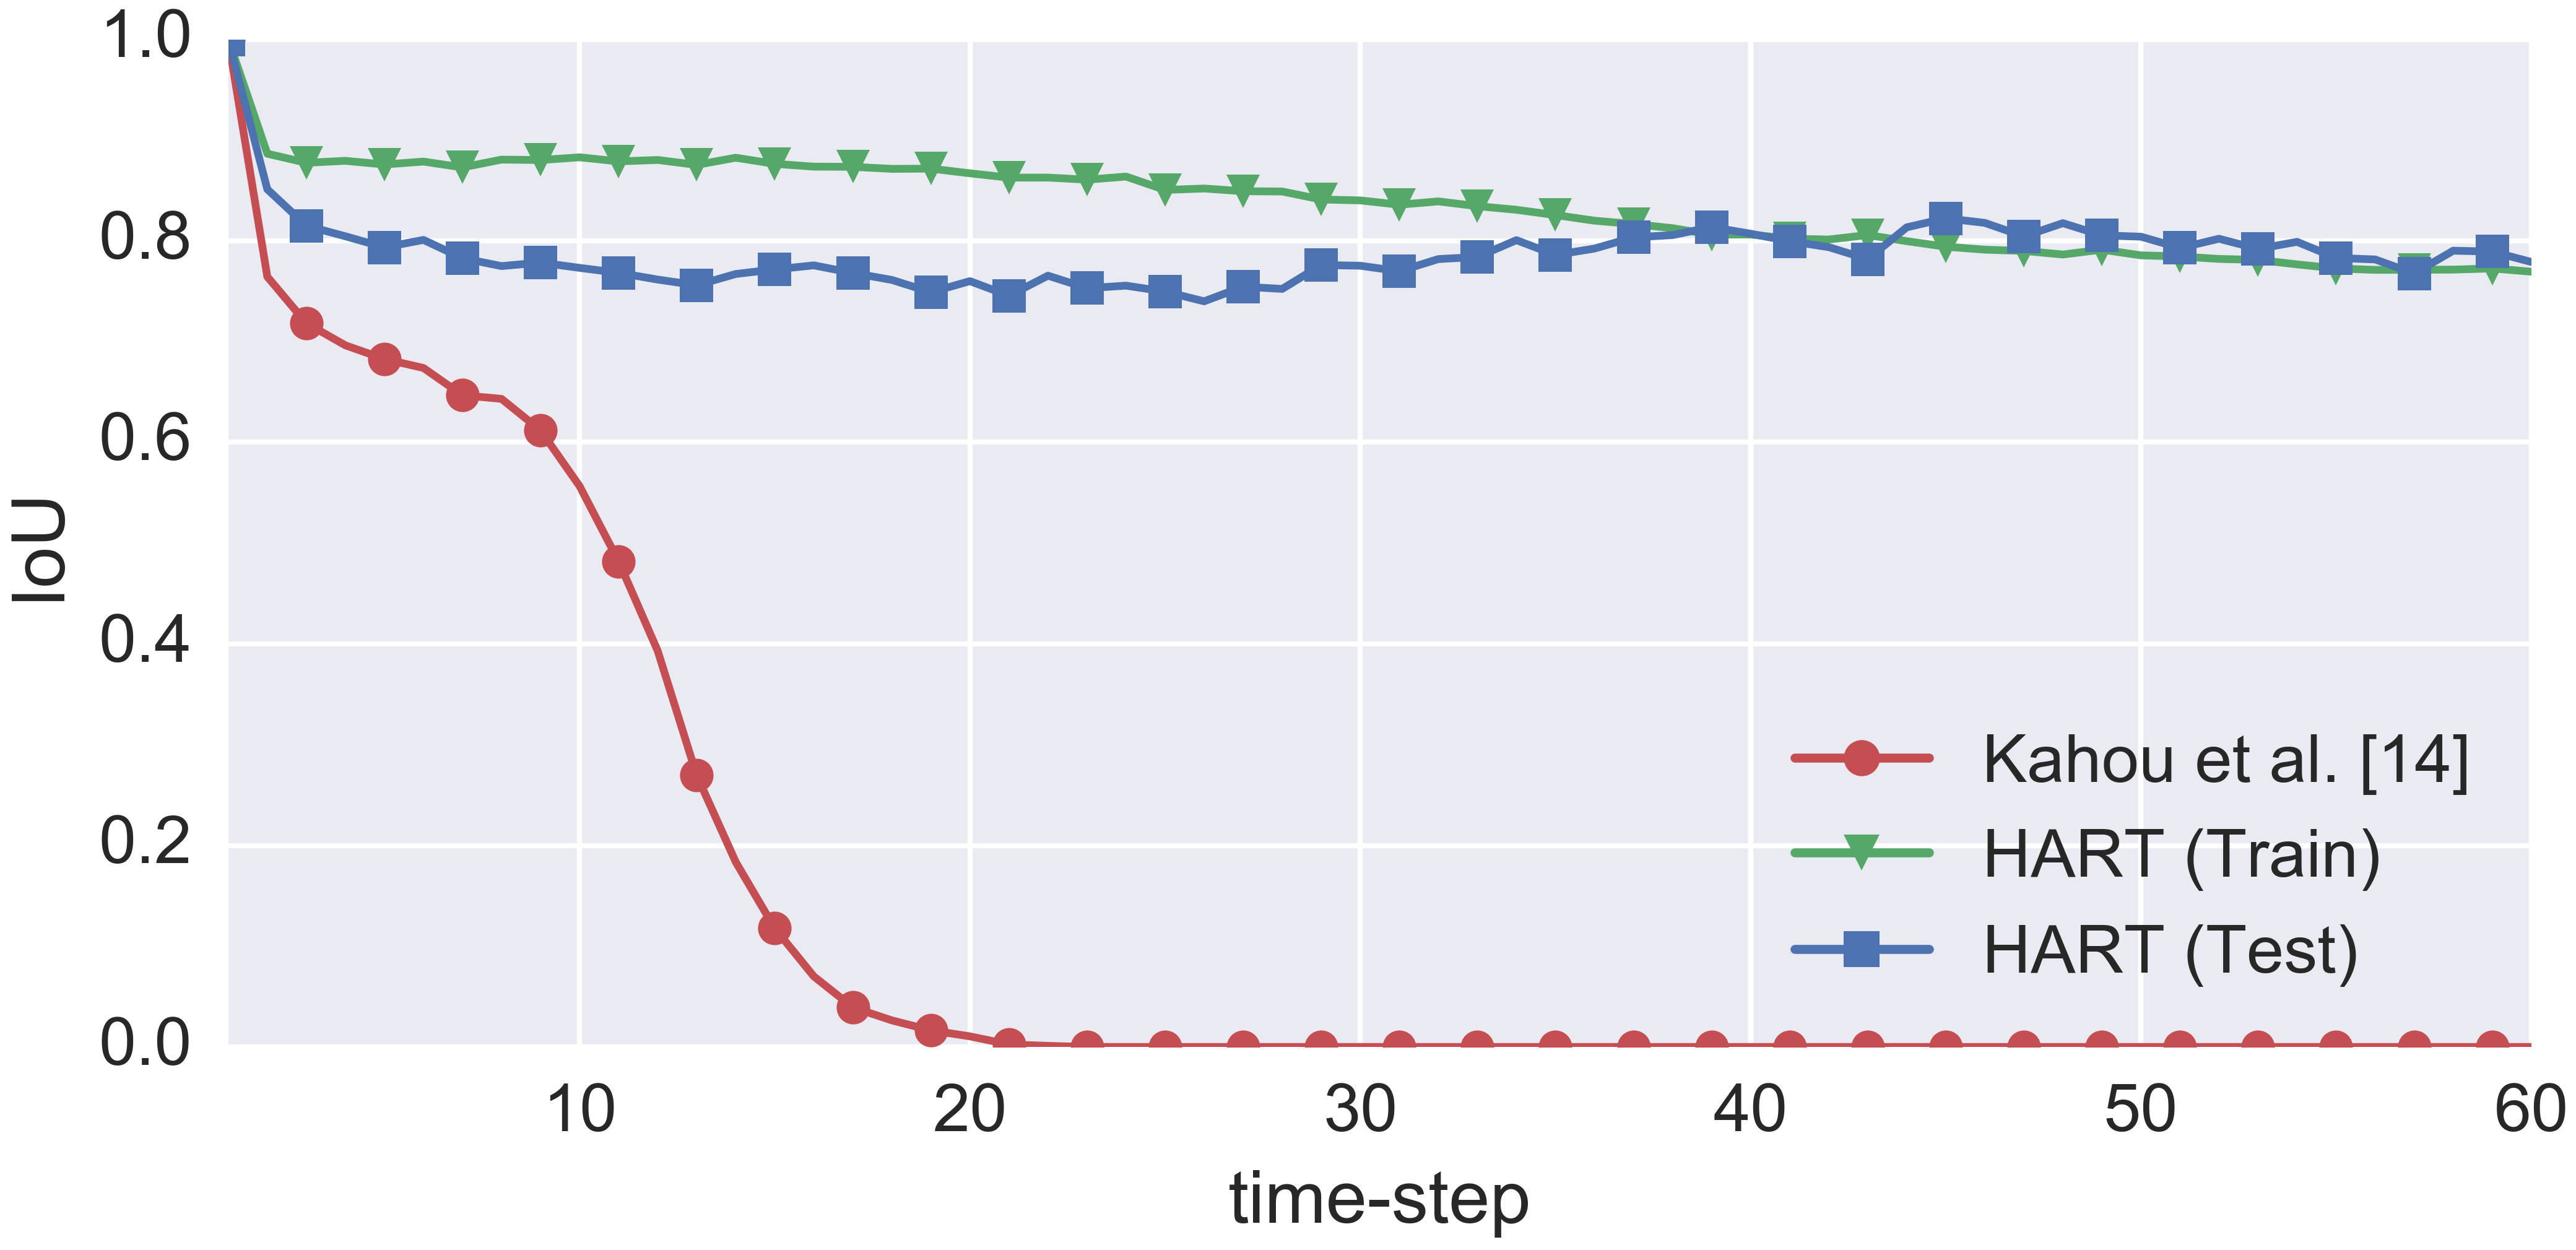
\includegraphics[width=\textwidth]{kitti_iou_fig}
        
        {\large
        \begin{minipage}[c]{0.5\linewidth}
            \centering
            \begin{tabular}{c|c|c|c}
                \multicolumn{4}{c}{Average IoU on KITTI over 60 time-steps}\\
                Kahou \emph{et. al.} [1] & Spatial Att & App Att & HART\\
                \midrule
                0.14 & 0.60 & 0.78 & \B{0.81}
            \end{tabular}
        \end{minipage}
        }\hfill
        \begin{minipage}[c]{0.4\linewidth}
            IoU curves on KITTI over 60 timesteps. HART~(train) presents evaluation on the train set.
        \end{minipage}
    \end{minipage}
    

    \vspace{1em}


%        \begin{tabular}{c|c}
%            \toprule
%            Method                      &   Avg. IoU\\
%            \midrule
%            \citet{Kahou2015ratm}       &   0.14      \\
%            Spatial Att                 &   0.60       \\  
%            % 			Spatial Att with Loss       &   0.70   \\
%            App Att                     &   0.78       \\
%            HART                        &   \B{0.81}   \\
%            \bottomrule
%        \end{tabular}
%        \vspace{1em}
%        Average IoU on KITTI over 60 time-steps.

\mysection{Conclusion}

\begin{description}[labelsep=1em, leftmargin=!,labelwidth=\widthof{\bfseries Interpretable:}]
    \item[Bio-inspired:] Neural Recurrent tracking with\\ Attention Mechanisms.
    \item[Interpretable:] Important features selected by spatial attention and object segmentation mechanisms.
    \item[Scalable:] Auxiliary loss terms allow scaling to\\ complex real-world datasets.
    \item[Efficient:] $> 120$ fps on a laptop! 
    \item[Future Work:] Multi-object tracking.
\end{description}

%\small{
%\bibliographystyle{unsrt}
%\bibliographystyle{../misc/natbib}
%\bibliography{../misc/library,../misc/biblio,../misc/bibdesk-porbanz}
%}

\end{multicols}

\end{poster}

\end{document}
